\section{Nonlinear multi-observers}\label{ch:nonlinear-mos}
In this chapter the issues with MOs applied on nonlinear systems will be discussed. We will employ an MO on system \eqref{eqn:standard-system} which will be repeated here for clarity
\begin{equation*}
    \begin{split}
        \dot{x}(t) &= Ax(t) + Bu(t) + E\phi(x) \\
        y_i(t) &= C_ix(t) + Du(t) + v_i(t) + \tau_i(t) \quad i \in \mathcal{N} = \{1,2,\dots,N_O\}.
    \end{split}
\end{equation*}
First the observers will be extended with the aim of correctly observing the state of system \eqref{eqn:standard-system} when less then half of the sensors are under attack (the same boundary condition as discussed in Chapter \ref{ch:cmo}).

\subsection{Extending the state-estimates}
Let us extend the MO to also observe nonlinear systems as a single observer in Equation \eqref{eqn:nonlinear-single-observer}. Let us extend the observers as in Equations \eqref{eqn:cmo-single-J-observer}
\begin{equation}\label{eqn:nonlinear-mo}
    \begin{split}
        \dot{\hat{x}}_{j/p}^{\mcJ/\mcP} &= (A + L_{j/p}^{\mcJ/\mcP}C_{j/p}^{\mcJ/\mcP})\hat{x}^{\mcJ/\mcP}_{j/p} - L_{j/p}^JC_{j/p}^{\mcJ/\mcP}x + Bu + E\phi(y) - L_{j/p}^{\mcJ/\mcP}(v_{j/p}^{\mcJ/\mcP} + \tau_{j/p}^{\mcJ/\mcP}),
    \end{split}
\end{equation}
where $j=1,2,\dots,N_J$, $p=1,2,\dots,N_P$ and $j/p$ indicates that the equation holds for both $J$ and $P$-observers. The resulting observer in Equation \ref{eqn:nonlinear-mo} is analogous to the observer in \cite[Equation 5]{Chong2023MemoryAlgorithms}. In this case the nonlinearity is output dependent, the full $y$ is used as input and not the subset that corresponds to the the specific $p$ or $j$. This has some implications in the SSE context, where some $y_i$ are corrupted. If the $y_i$ that happen to be used by the nonlinearity $\phi(y)$ is attacked, all state estimates become corrupted. So no 

\begin{example}\label{ex:nonlinear-issue}
    Let us work through an example to clarify this issue, consider system \eqref{eqn:example-system} as defined in Example \ref{ex:system}, where we change $C$ to have $N_O=6$ outputs
    \begin{equation}\label{eqn:NL-ex-C-6out}
        C = 
        \begin{bmatrix}
            1 & 0 & 0 & 0 \\
            1 & 0 & 1 & 0 \\
            1 & 0 & 0 & 0 \\
            1 & 0 & 1 & 0 \\
            1 & 0 & 0 & 0 \\
            1 & 0 & 1 & 0 \\
        \end{bmatrix}.
    \end{equation}
    This means there are 3 copies of each sensor. The nonlinear spring as in Equation \eqref{eqn:nonlinear-spring} uses the spring constants and positions of each individual mass as input. Since we now have three copies of each position sensor we can select any combination of two sensors measuring a different position. Let us select the first two sensors, $y_1$ and $y_2$. We now construct
    \begin{equation}\label{eqn:NL-ex-phi-6out}
        \phi(y) = 
        \begin{bmatrix}
            F^{NL}_s(y_1) \\ F^{NL}_s(y_2) \\
        \end{bmatrix},
    \end{equation}
    which leads to the following $E$ matrix
    \begin{equation}\label{eqn:NL-ex-E-6out}
        E =
        \begin{bmatrix}
            0 & 0 \\
            -1 & 1 \\
            0 & 0 \\
            0 & -1 \\
        \end{bmatrix}.
    \end{equation}
    Figure \ref{fig:nonlinear-functional} displays a scenario where $\mathcal{M}=\{3,6\}$, so outputs $3$ and $6$ are under attack, with the attack signal $\tau_k=t,k \in \mathcal{M}$ The MO works as expected and provides a correct state estimate. The $\phi(y)$ provides a correct value for all $t \geq 0$.
    \begin{figure}[H]
        \centering
        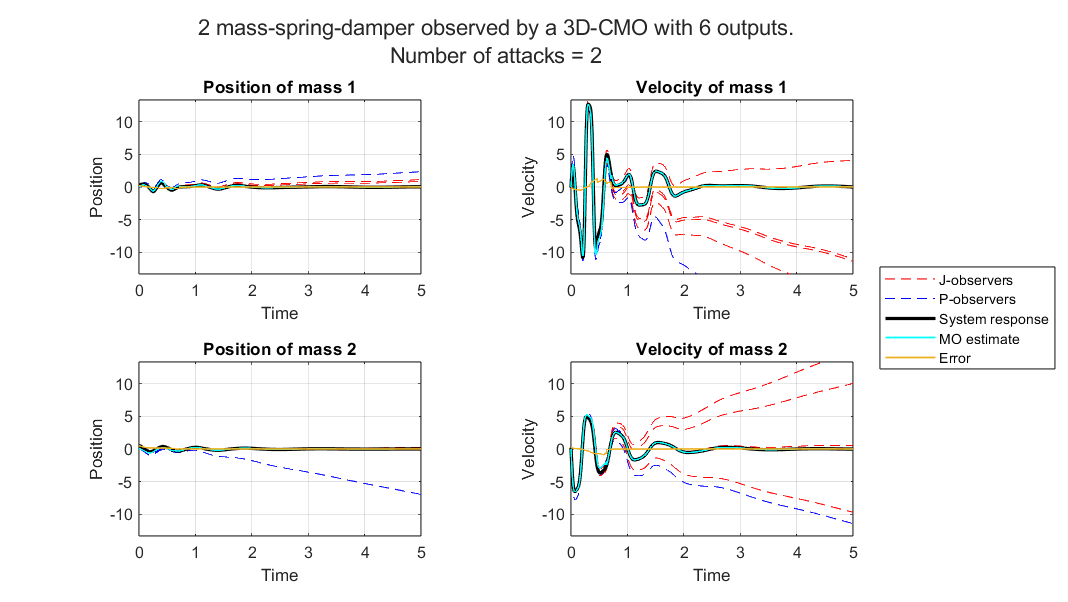
\includegraphics[width=\linewidth]{report/Figures/nonlinear_functional.png}
        \caption{Nonlinear double mass-spring-damper model with outputs $3$ and $6$ under attack.}
        \label{fig:nonlinear-functional}
    \end{figure}
    Figure \ref{fig:nonlinear-not-functional} shows a scenario where $\mathcal{M}=\{1,4\}$. Or in other words, outputs $1$ and $4$ are under attack. The attack signal is the same as in the previous case, $\tau_k=t,k \in \mathcal{M}$. All state estimates fail in this case, because $\phi(y)$ uses an attacked output.

    \begin{figure}[H]
        \centering
        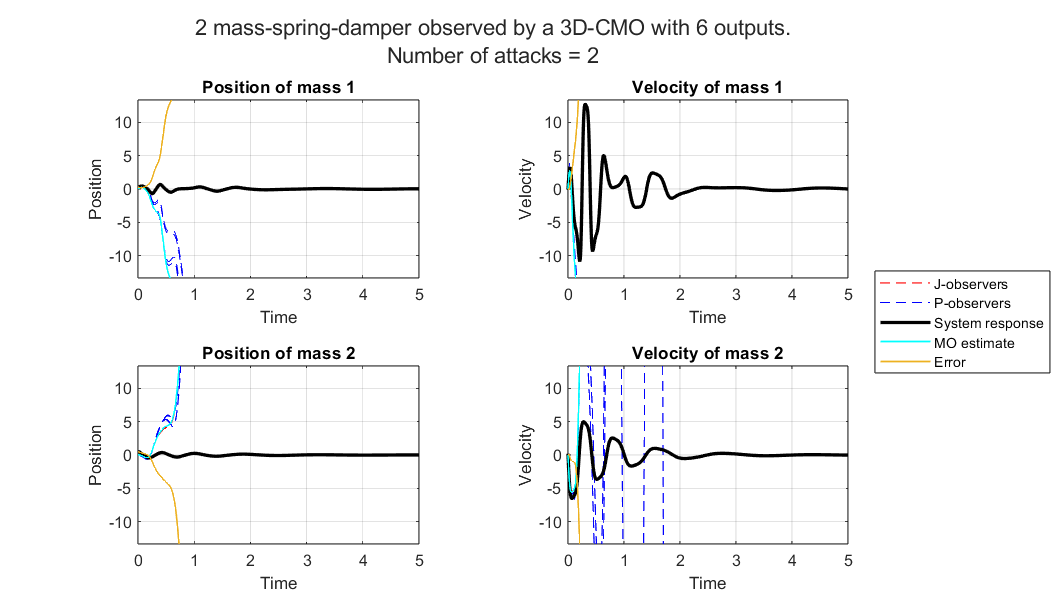
\includegraphics[width=\linewidth]{report/Figures/nonlinear_not_functional.png}
        \caption{Nonlinear double mass-spring-damper model with outputs $1$ and $4$ under attack.}
        \label{fig:nonlinear-not-functional}
    \end{figure}
\end{example}

Both Figures \ref{fig:nonlinear-functional} and \ref{fig:nonlinear-not-functional} show the result of a 3D-CMO, the result on an SSMO is the same. Not surprising, since they realize the same set of observers.

\subsection{Addressing the nonlinear issue}
As discussed in Example \ref{ex:nonlinear-issue} the issue arises because the observers' nonlinear extension does not employ any intelligent logic in choosing which outputs are used to calculate the nonlinear contribution. The nonlinearity $\phi(y)$ should either 'know' which $y_i$ are corrupted and avoid them, which is contradictory with the demands of SSE. Or it should be able to provide a correct state estimate even with an unknown subset of sensors under attack. Let us now discuss the implications and difficulties of this issue for both the 3D-CMO and the SSMO, we will not consider the 2D-CMO in this section. 

Let us start with the SSMO, the shared state is calculated as in Equation \eqref{eqn:ssmo-z} which we repeat for readability
\begin{equation*}
    \dot{z} = \mathbf{A}z + \mathbf{B}\eta, \quad \eta = 
    \begin{bmatrix}
        u \\ y
    \end{bmatrix}.
\end{equation*}
The nonlinearity no longer appears in this structure, since it is taken into account during construction of the shared $\mathbf{B}$ matrix. The input to the nonlinear function $\phi(y)$ is also 'hidden' behind the shared state. We cannot try different combinations of sensors $y_i$ because we only calculate a single state $z$, which uses a single external input $\eta$ with the full output $y$.

We now continue with the 3D-CMO, which has more control over each individual state estimate $\hat{x}^{\mcJ/\mcP}_{j/p}$. Since every observer is calculated separately, a different nonlinear contribution can be used for every observer
\begin{equation}\label{eqn:ext-NL-observer}
    \begin{split}
        \dot{\hat{x}}_{j/p}^{\mcJ/\mcP} &= (A + L_{j/p}^{\mcJ/\mcP}C_{j/p}^{\mcJ/\mcP})\hat{x}^{\mcJ/\mcP}_{j/p} - L_{j/p}^JC_{j/p}^{\mcJ/\mcP}x + Bu + E\phi(y^{\mcJ/\mcP}_{j/p}) - L_{j/p}^{\mcJ/\mcP}(v_{j/p}^{\mcJ/\mcP} + \tau_{j/p}^{\mcJ/\mcP}).
    \end{split}
\end{equation}
The nonlinear contribution $E\phi(y^{\mcJ/\mcP}_{j/p})$ uses the subset $j$ or $p$ as input to the function $\phi(y)$. Let us work out two examples that clarify some of the implications this extended 3D-CMO has. We start with an example that investigates a system where $\phi(y)$ is dependent only on one measured state variable.

\begin{example}\label{ex:single-mass-nonlinear-example}
    Consider the system as in Equation \eqref{eqn:standard-system} with system matrices
    \begin{equation*}
        A =
        \begin{bmatrix}
            0 & 1 \\ -15 & -2 \\
        \end{bmatrix}, \quad
        B =
        \begin{bmatrix}
            0 \\ 1 \\
        \end{bmatrix}, \quad
        C = 
        \begin{bmatrix}
            1 & 0 \\ 1 & 0 \\ 1 & 0 \\ 1 & 0 \\ 1 & 0 \\
        \end{bmatrix}, \quad
        D = 0, \quad
        E =
        \begin{bmatrix}
            0 \\ -1 \\
        \end{bmatrix},   
    \end{equation*}
    as derived from the general mass-spring-damper described in Chapter \ref{ch:system-definition}.  The nonlinearity looks like
    \begin{equation*}
        \phi(y^{\mcJ/\mcP}_{j/p}) = F^{NL}_s((y^{\mcJ/\mcP}_{j/p})_1),
    \end{equation*}
    where the subscript $1$ indicates the first element of $y^{\mcJ/\mcP}_{j/p}$. The system has $N_O=5$ outputs, let us attack $N_M=2$ of those outputs. $\mathcal{M}=\{2,4\}$, so outputs $2$ and $4$ are under attack. Again the attack signal $\tau_k=t,k \in \mathcal{M}$ is used. Figure \ref{fig:single-nonlinear-functional} shows the result of such an attack, the MO successfully estimates the state and the error approaches zero. 
    \begin{figure}[H]
        \centering
        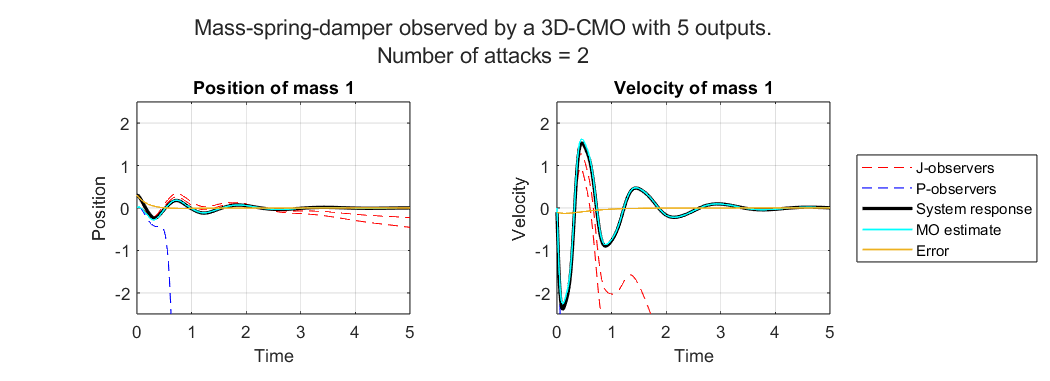
\includegraphics[width=\linewidth]{report/Figures/single-nonnlinear-functional.png}
        \caption{Single nonlinear mass-spring-damper with outputs $2$ and $4$ under attack.}
        \label{fig:single-nonlinear-functional}
    \end{figure}
    In this scenario the MO functions because all sensors measure the same variable, the position of the first (and only) mass. So the combination $j=\{1,3,5\}$ provides a successful state estimate because $\phi(y_1)=\phi(y_3)=\phi(y_5)=\phi(\begin{bmatrix}y_1&y_3&y_5\end{bmatrix}^T)$. 
\end{example}
Let us now investigate a scenario where the nonlinearity $\phi(y)$ depends on multiple measured state variables.

\begin{example}\label{ex:ext-NL-double-mass}
    Now, consider the same system \eqref{eqn:example-system} as in Example \ref{ex:system}, where $C$ is changed to have $N_O=5$
    \begin{equation*}
        C = 
        \begin{bmatrix}
            1 & 0 & 0 & 0 \\
            1 & 0 & 1 & 0 \\
            1 & 0 & 0 & 0 \\
            1 & 0 & 1 & 0 \\
            1 & 0 & 0 & 0 \\
        \end{bmatrix}.
    \end{equation*}
    Let us now choose $N_M=2$ in order to still satisfy the $N_O>2N_M$ requirement. Where we specify $\mathcal{M}$ as $\{2,4\}$, note that now all copies of the sensor measuring the position of mass 2 are attacked. Figure \ref{fig:extended_nonlinear_not_functional} shows that the error $\hat{x}-x$ still approaches $0$ as $t$ increases. But the estimates, especially of the velocities, do not look to be tracking the true state correctly.
    \begin{figure}[H]
        \centering
        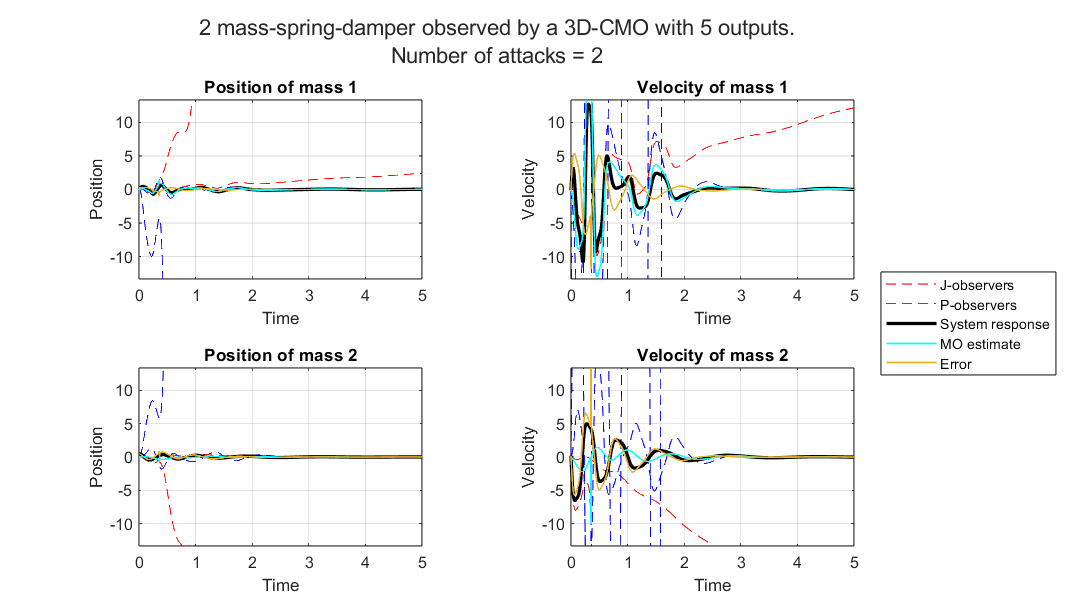
\includegraphics[width=\linewidth]{report/Figures/extended_nonlinear_not_functional.png}
        \caption{Double nonlinear mass-spring-damper with outputs 2 and 4 under attack.}
        \label{fig:extended_nonlinear_not_functional}
    \end{figure}
    Let us now expand the number of outputs to $N_O=6$, and use the exact same system as in Equations \eqref{eqn:NL-ex-C-6out},\eqref{eqn:NL-ex-E-6out} and \eqref{eqn:NL-ex-phi-6out} as in Example \ref{ex:nonlinear-issue}. We now use the observer as in Equation \eqref{eqn:ext-NL-observer} and attack the system with the attack signal $\tau_k=t,k \in \mathcal{M},\mathcal{M}=\{4,6\}$ \textcolor{red}{ugly}.
    \begin{figure}[H]
        \centering
        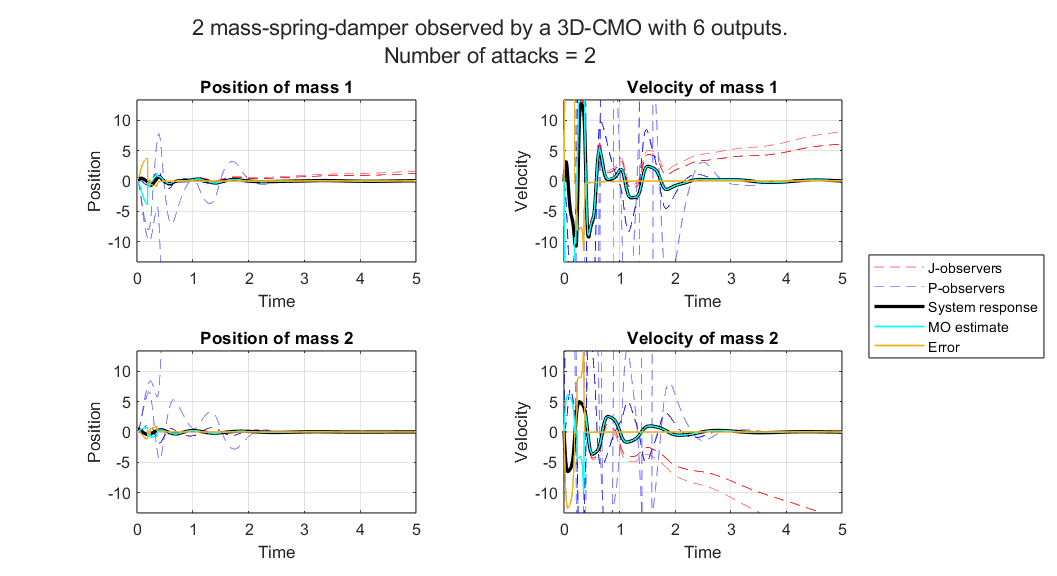
\includegraphics[width=\linewidth]{report/Figures/extended-nonlinear-functional.png}
        \caption{Double mass-spring-damper with outputs $4$ and $6$ under attack.}
        \label{fig:extended-nonlinear-functional}
    \end{figure}
    The state estimates in Figure \ref{fig:extended-nonlinear-functional} look to be tracking the true state much better. The MO now functions correctly because the state estimate using $j=\{1,2,3,5\}$ has the uncorrupted outputs $1$ and $2$ as input to $\phi(y)$ as in Equation \eqref{eqn:NL-ex-phi-6out}.
\end{example}
The attacked outputs in Example \ref{ex:ext-NL-double-mass} have, of course, been carefully chosen to provide the correct results. Had we attacked outputs $2$ and $4$ in the $N_O=6$ case, no correct state estimate could have been provided. This happens because in the setup in the example $\phi(y)$ takes the first two entries of $y^{\mcJ/\mcP}_{j/p}$ irrespective of what the sensor measures. So if outputs $2$ and $4$ are attacked, even the fully uncorrupted set of outputs $j=\{1,3,5,6\}$ does not provide a correct state estimate. Because $\phi(y)$ is only considers outputs $1$ and $3$ in this state estimate. If we provide the reading of sensor $6$ in the second position, the nonlinearity would use the correct input value. For a double mass-spring-damper system the outputs could be sorted to feature uneven and even sensors in an alternating pattern, as long as possible. For the set we are considering now, it could take the form $\{1,6,3,5\}$ \textcolor{red}{how to denote ordered sets?}. In order to generalize this method for systems with a nonlinearity depending on $n$ variables the list should be sorted based on multiples... \textcolor{red}{if this stays in needs to much more detailed}

Up till now, only the $J$-observers have been discussed. Let us use the set of outputs $j=\{1,3,5,6\}$ again. During the final estimate selection procedure as described in subsection \ref{subsec:estimate-selection}. All estimates constructed with $p \in j$ are compared against the estimate constructed with $j$. We now encounter the same pitfall as before: for all sizes of $p$ that are smaller then $|j|$, some possible subsets do not contain any sensor measuring the position of the second mass.